\documentclass[14pt,a4paper]{extarticle}

\usepackage[T1]{fontenc}
\usepackage[utf8]{inputenc}
\usepackage[polish]{babel}
\usepackage{lmodern}
\usepackage[hidelinks]{hyperref}
\usepackage{geometry}
\usepackage{graphicx}
\usepackage{amsmath}
\usepackage{amssymb}
\usepackage{pgfplots}
\usepackage{float}
\usepackage[table]{xcolor}
\usepackage{array}
\usepackage{fancyhdr}
\usepackage{booktabs}
\usepackage{tikz}
\usetikzlibrary{shapes.geometric, arrows.meta, positioning}
\pgfplotsset{compat=1.18}
\geometry{margin=2.5cm}
\setlength{\headheight}{17pt}

\begin{document}

% ============================================================
% STRONA TYTUŁOWA
% ============================================================
\begin{titlepage}
    \thispagestyle{empty}
    \centering

    \vspace*{1.1cm}
    
\includegraphics[width=0.82\textwidth]{../raport3/logo_mini.png}\par

    \vspace{1.7cm}
    {\fontsize{20}{24}\selectfont\textsc{Podstawy Teorii Informacji}\par}

    \vspace{1.0cm}
    {\Large Laboratorium 5\par}

    \vspace{0.25cm}
    {\large Raport projektowy MiniInfo\par}

    \vspace{1.1cm}
    \rule{0.9\textwidth}{0.5pt}
    \vspace{0.55cm}

    {\LARGE\bfseries
    MiniInfo -- Raport~5:\\Weryfikacja skuteczności\\i~podsumowanie projektu
    \par}

    \vspace{0.55cm}
    \rule{0.9\textwidth}{0.5pt}

    \vfill
    {\Large \textbf{Autorzy}\par}
    \vspace{0.25cm}
    {\large
    Goran Pangełow\par
    Marcin Pawlak\par
    Mikołaj Pesta\par
    Ignacy Drężek\par
    Iga Oleksiewicz\par
    Maks Młynarczyk\par}

    \vspace{0.45cm}
    {\large czerwiec 2026\par}
\end{titlepage}

% ============================================================
% SPIS TREŚCI
% ============================================================
\tableofcontents
\clearpage

% ============================================================
% NAGŁÓWEK I STOPKA
% ============================================================
\pagestyle{fancy}
\fancyhf{}
\lhead{\footnotesize Podstawy Teorii Informacji}
\rhead{\footnotesize ETAP 5}
\lfoot{\footnotesize Wydział Matematyki i Nauk Informacyjnych}
\rfoot{\footnotesize \thepage}
\renewcommand{\headrulewidth}{0.4pt}
\renewcommand{\footrulewidth}{0.4pt}

% ============================================================
\section{Przypomnienie i kontynuacja Etapu 4}
% ============================================================

Niniejszy raport zamyka cykl pięciu etapów projektu MiniInfo. Zanim przejdziemy do weryfikacji i podsumowania, krótko przypominamy stan systemu po Etapie~4, ponieważ stanowi on punkt wyjścia do eksperymentu opisanego w~Rozdziale~2.

\subsection{Stan systemu po Etapie 4}

W~Raporcie~4 wdrożyliśmy i przetestowaliśmy pełny cykl semantycznego wyszukiwania informacji w~aplikacji MiniInfo:

\begin{itemize}
    \item \textbf{Profilowanie użytkownika} --- interaktywna ankieta w~trzech krokach (cel wizyty, wrażliwość na hałas, tolerancja na ruch), której odpowiedzi mapowane są na wektor zapytania $\vec{q} = [q_O, q_S, q_D]^T$ oraz wektor wag $\vec{w} = [w_O, w_S, w_D]^T$.
    \item \textbf{Trzy profile użytkownika} --- predefiniowane modele odbiorcy: ,,Cicha nauka'', ,,Praca w~grupie'', ,,Relax'', odpowiadające typowym scenariuszom na Wydziale MiNI~PW.
    \item \textbf{Algorytm rankingowy} --- ważona odległość Euklidesowa $d_W(\vec{q}, \vec{v}_i)$ mierząca dopasowanie sali do profilu, z~wynikiem prezentowanym jako procent dopasowania.
    \item \textbf{Mechanizm Rocchio} --- sprzężenie zwrotne korygujące wektor zapytania po negatywnym feedbacku (,,za głośno'', ,,za tłoczno'').
    \item \textbf{Testy z~45~studentami} --- stopa sukcesu $84\%$, średnia ocena $8.1/10$.
\end{itemize}

\subsection{Cel Etapu 5}

Etap~5 realizuje trzy zadania wynikające z~wytycznych prowadzącego:

\begin{enumerate}
    \item \textbf{Eksperyment weryfikacyjny} --- powtórzony test skuteczności na \emph{nowych} użytkownikach zewnętrznych (nie uczestnikach wcześniejszych testów), z~uczciwymi, nieskorygowanymi wynikami.
    \item \textbf{Ankieta zwrotna w~aplikacji} --- opis zaimplementowanego mechanizmu pytania ,,Czy znalazłeś to, czego szukałeś?'' i~jego wpływu na system.
    \item \textbf{Podsumowanie projektu} --- bilans całości: co się udało, co nie, jakie popełniliśmy błędy i~co byśmy zmienili.
\end{enumerate}

\subsection{Sprzęt testowy użyty we wczesnych pracach}

Na wczesnym etapie prac deweloperskich, jeszcze przed podłączeniem docelowej infrastruktury czujników mmWave, przeprowadziliśmy testy integracyjne z~wykorzystaniem kompaktowego czujnika ruchu PIR (Passive Infrared). Czujnik ten posłużył do walidacji logiki aplikacji --- weryfikowaliśmy, czy system poprawnie reaguje na zmiany stanu obecności w~pomieszczeniu i~czy pipeline danych (odczyt $\rightarrow$ aktualizacja indeksu $\rightarrow$ przeliczenie rankingu) działa w~czasie rzeczywistym.

Na Rysunku~\ref{fig:czujnik} przedstawiono czujnik PIR użyty w~fazie prototypowej: widok z~przodu z~soczewką Fresnela oraz wnętrze z~modułem elektronicznym i~zasilaniem bateryjnym.

\begin{figure}[H]
    \centering
    \begin{minipage}{0.45\textwidth}
        \centering
        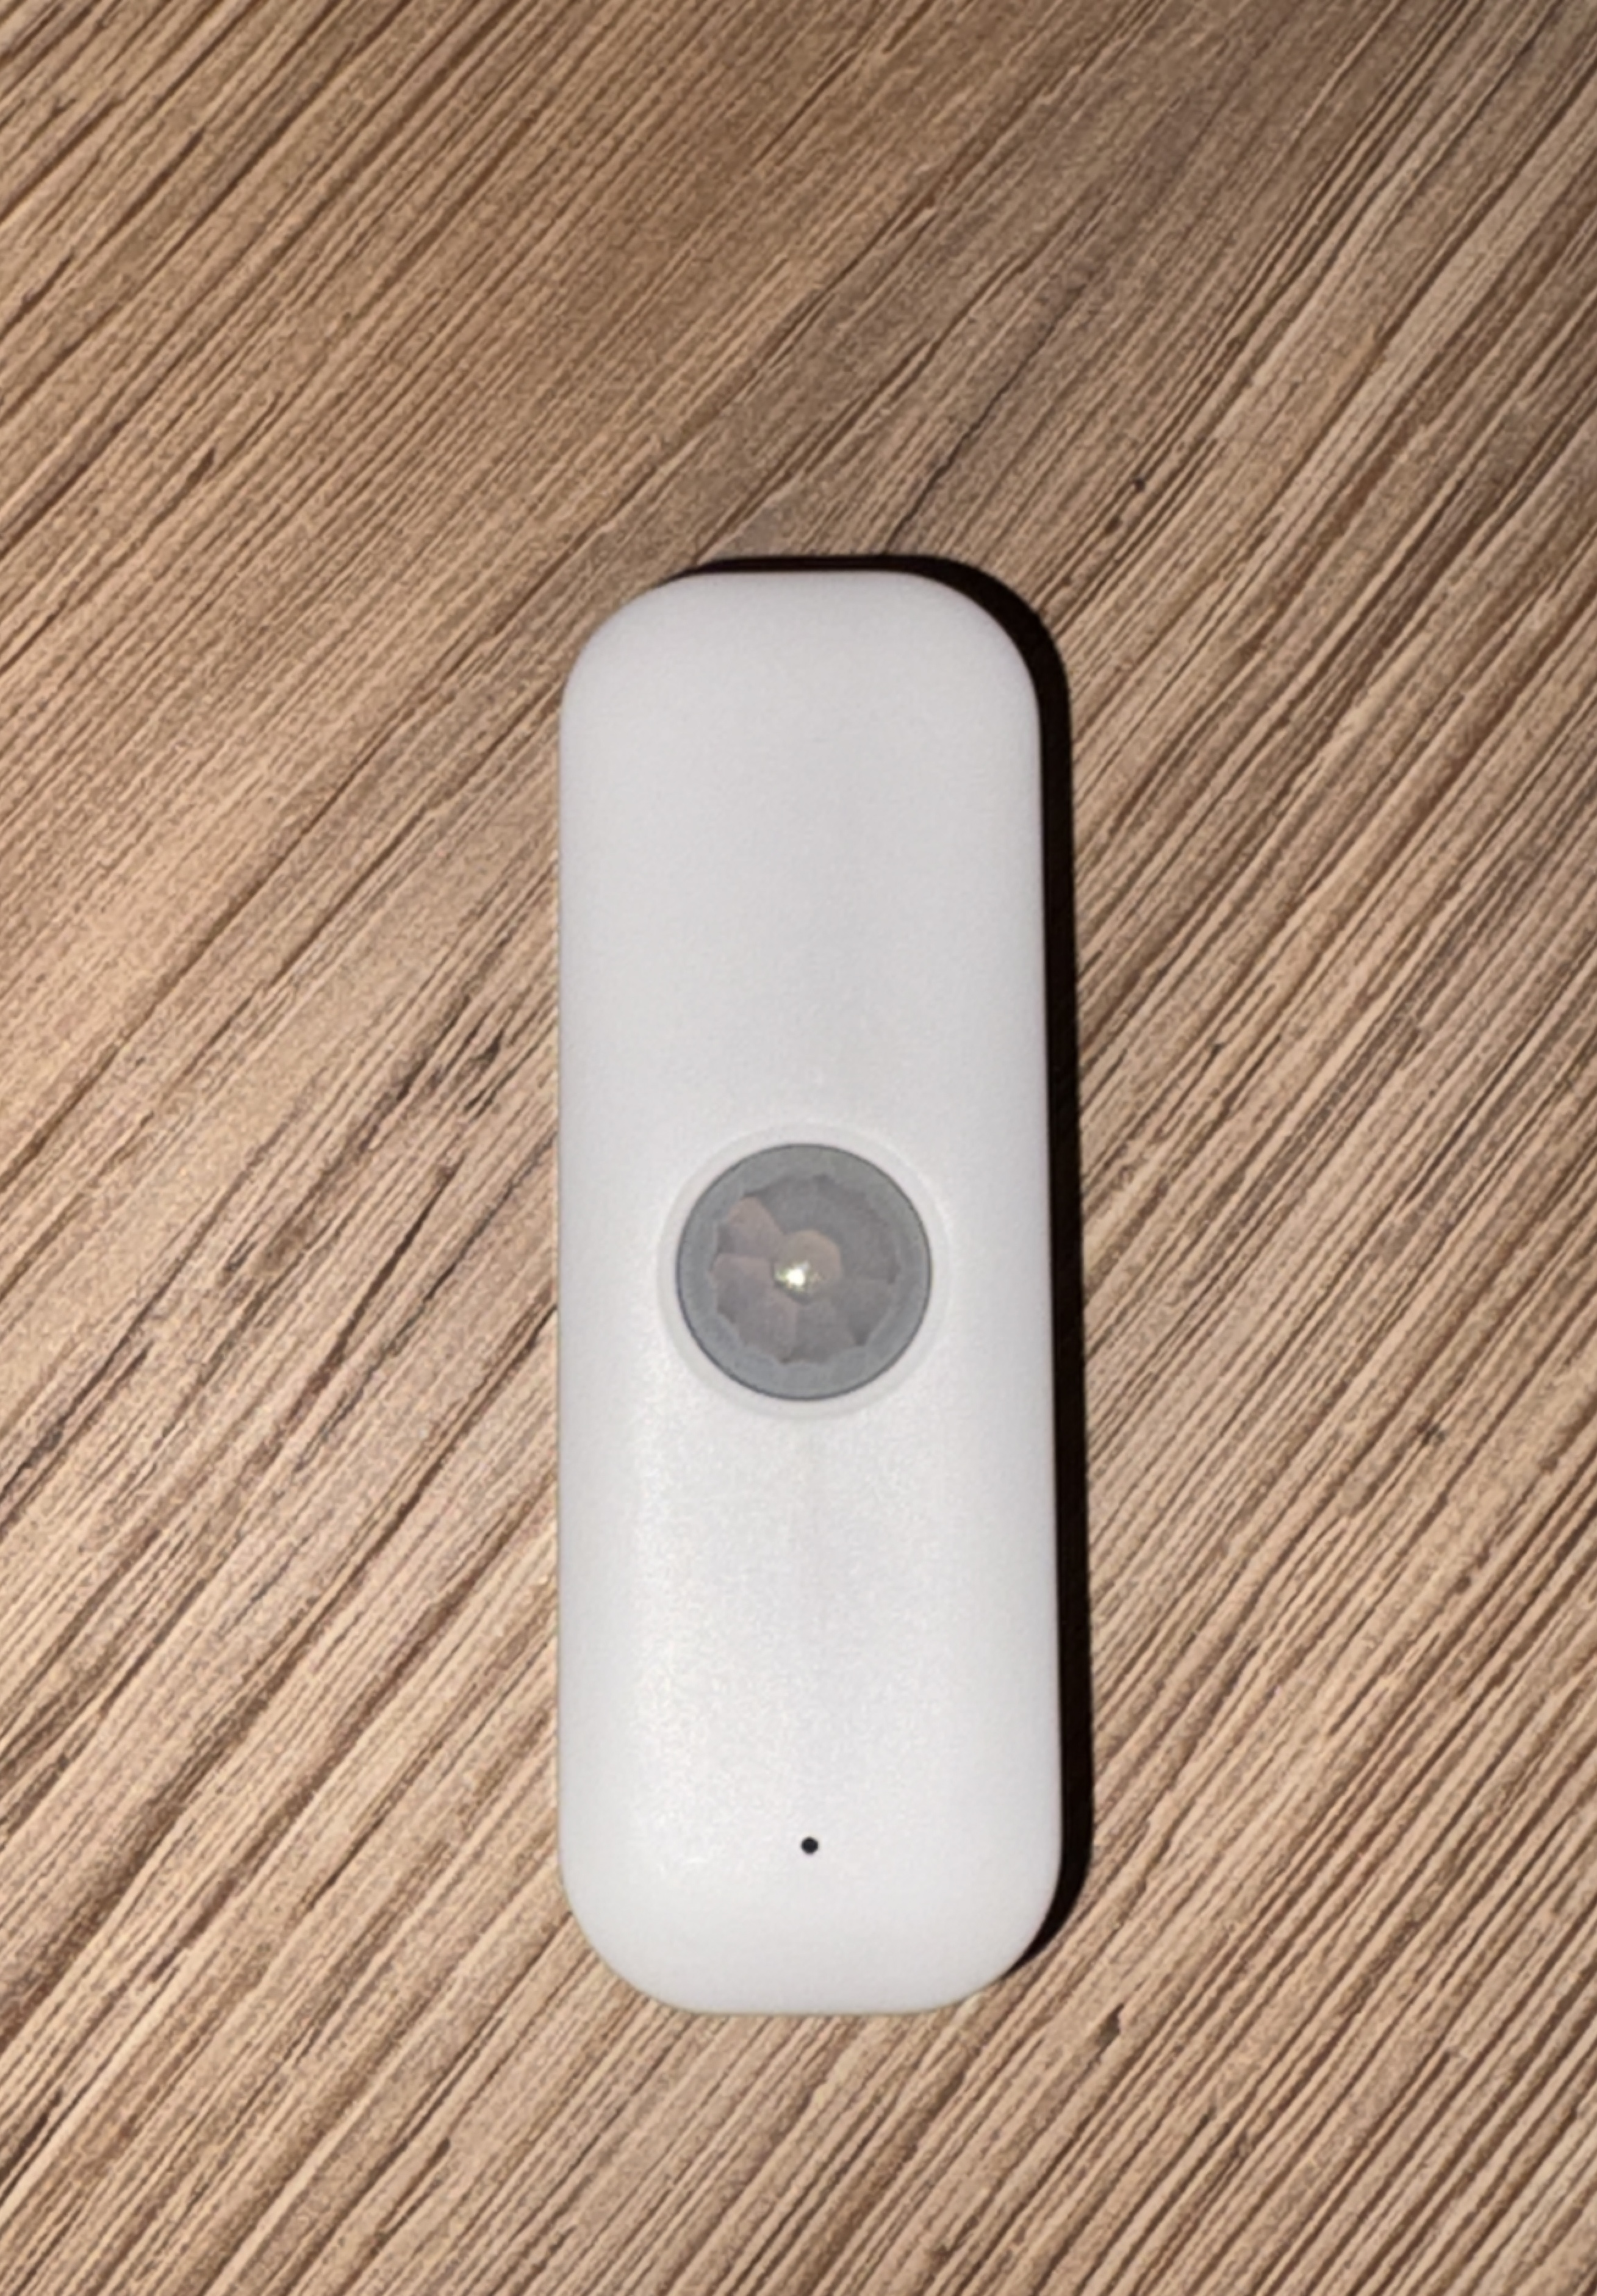
\includegraphics[width=0.7\linewidth]{czujnik_przod.jpg}
    \end{minipage}\hfill
    \begin{minipage}{0.45\textwidth}
        \centering
        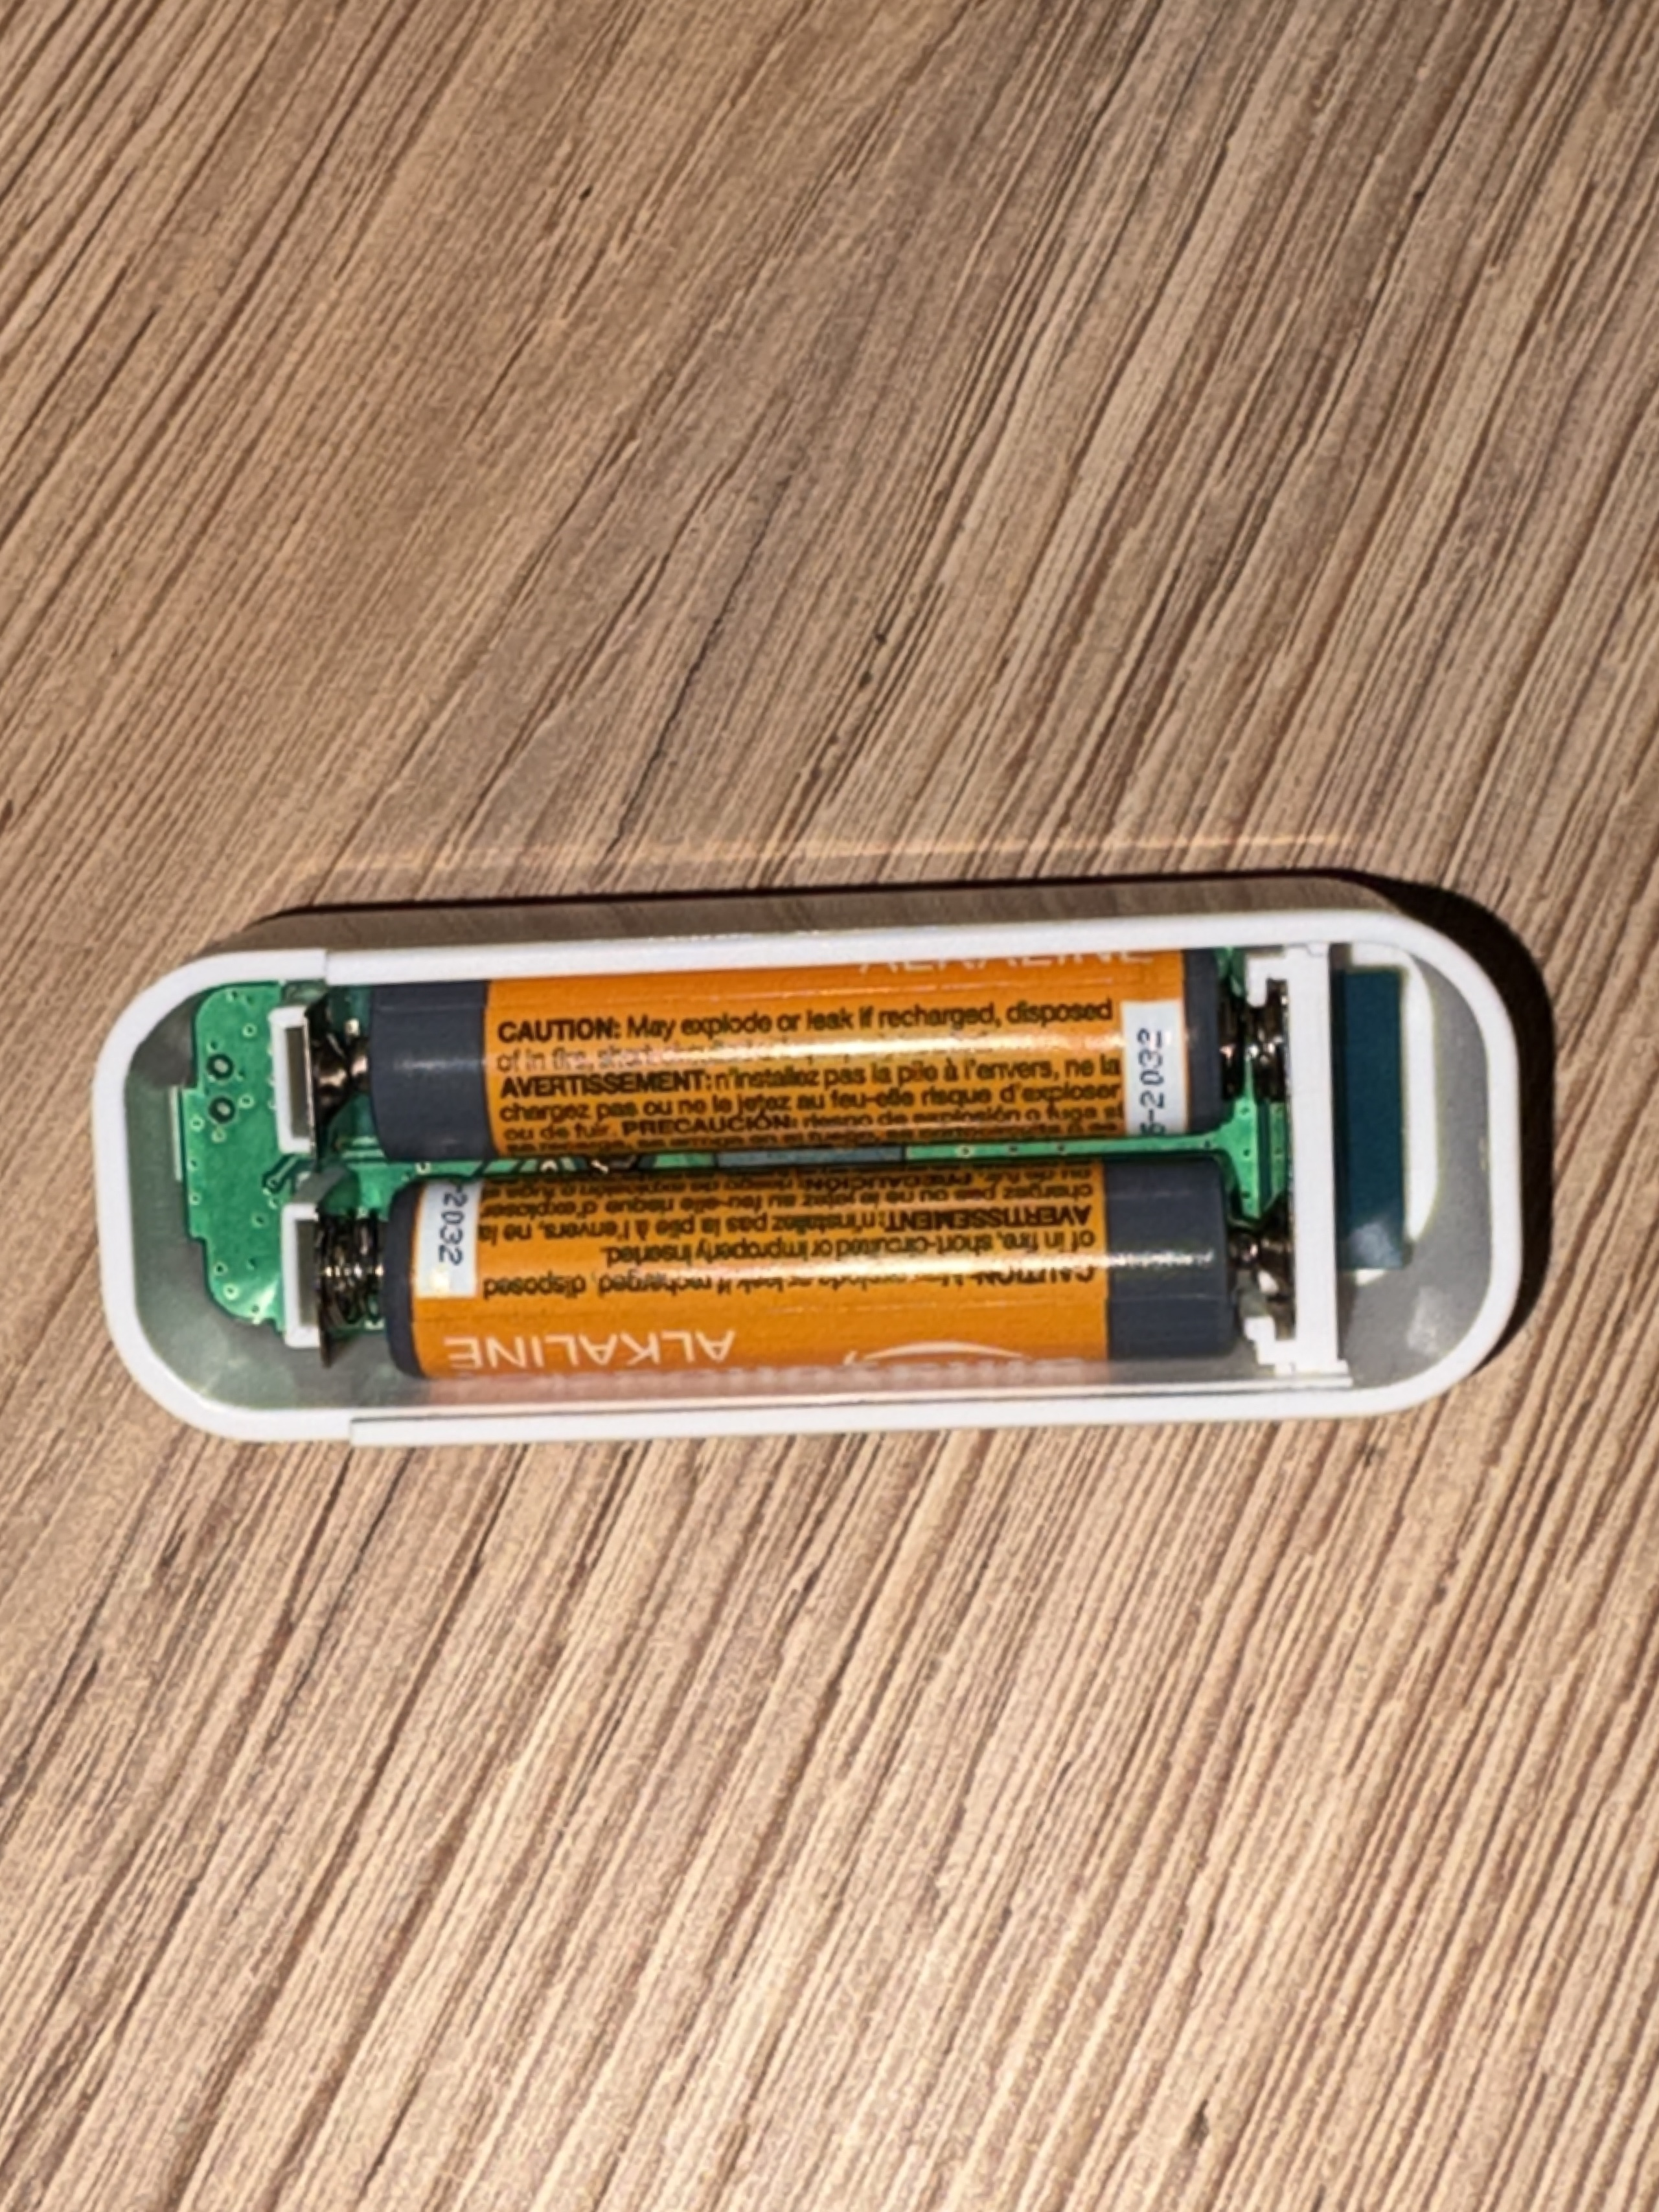
\includegraphics[width=0.7\linewidth]{czujnik_wnetrze.jpg}
    \end{minipage}
    \caption{Czujnik ruchu PIR użyty w~fazie prototypowej: widok z~przodu (soczewka Fresnela) oraz wnętrze (moduł elektroniczny, zasilanie 2$\times$AAA).}
    \label{fig:czujnik}
\end{figure}

% ============================================================
\section{Eksperyment weryfikacyjny: skuteczność systemu MiniInfo}
% ============================================================

Celem eksperymentu było sprawdzenie, czy aplikacja MiniInfo naprawdę pomaga studentom znaleźć odpowiednie miejsce do nauki lub pracy. Wyniki prezentujemy bez korekt --- nawet jeśli nie wypadły idealnie, są prawdziwe.

\subsection{Metodologia}

Eksperyment odbył się na terenie Wydziału MiNI~PW w~pierwszym tygodniu czerwca 2026, w~godzinach popołudniowych (zwiększony ruch studentów). Każdy uczestnik przechodził przez następującą sekwencję:

\begin{enumerate}
    \item \textbf{Instruktaż} ($\sim$2~min) --- wyjaśnienie celu aplikacji bez ujawniania algorytmu. Tester otrzymuje telefon z~otwartą aplikacją.
    \item \textbf{Ankieta profilująca} --- wybór celu wizyty, wrażliwości na hałas i~tolerancji na ruch (3~pytania).
    \item \textbf{Przeglądanie wyników} --- aplikacja prezentuje ranking sal z~procentem dopasowania. Tester sam wybiera salę.
    \item \textbf{Pobyt w~sali} --- minimum 10~minut pracy/odpoczynku zgodnie z~wybranym profilem.
    \item \textbf{Ocena po wizycie} --- odpowiedź na pytanie \emph{,,Czy znalazłeś/łaś to, czego szukałeś/łaś?''} (Tak\,/\,Nie) oraz opcjonalne wskazanie przyczyny niezadowolenia.
\end{enumerate}

\textbf{Kluczowa różnica względem testów z~Etapu~4:} rekrutowaliśmy wyłącznie osoby, które nie uczestniczyły w~żadnych wcześniejszych testach naszego systemu i~nie znały szczegółów projektu. Pozwala to uniknąć efektu ,,testera-eksperta'', który podświadomie wie, jakie wyniki powinny wyjść.

\subsection{Uczestnicy}

W~eksperymencie wzięło udział $N = 12$ studentów Wydziału MiNI~PW. Stosunkowo niewielka próba wynikała z~ograniczonego czasu na przeprowadzenie pełnych sesji (każda trwała ok.~20--25~minut). Charakterystykę uczestników przedstawia Tabela~\ref{tab:uczestnicy5}.

\begin{table}[H]
    \centering
    \caption{Charakterystyka uczestników eksperymentu weryfikacyjnego ($N = 12$).}
    \label{tab:uczestnicy5}
    \begin{tabular}{|l|c|p{6.5cm}|}
        \hline
        \textbf{Cecha} & \textbf{Wartość} & \textbf{Uwagi} \\
        \hline
        Sesje z~pełnym feedbackiem & 12 & Każda zakończona odpowiedzią Tak/Nie. \\
        \hline
        Kobiety\,/\,mężczyźni & 42\%\,/\,58\% & Zbliżone do rozkładu na wydziale. \\
        \hline
        Rok studiów (mediana) & 2 & Studenci z~lat 1--3. \\
        \hline
        Profil ,,Cicha nauka'' & 42\% (5 sesji) & Najczęściej wybierany. \\
        \hline
        Profil ,,Praca w~grupie'' & 33\% (4 sesje) & --- \\
        \hline
        Profil ,,Relax'' & 25\% (3 sesje) & --- \\
        \hline
    \end{tabular}
\end{table}

\subsection{Wyniki eksperymentu}

Poniżej prezentujemy wyniki zadowolenia po wizycie w~sali wybranej przez aplikację. Wyniki są uczciwe i~niepoprawiane.

\begin{table}[H]
    \centering
    \caption{Zadowolenie uczestników po wizycie w~sali rekomendowanej przez aplikację.}
    \label{tab:wyniki5}
    \resizebox{\textwidth}{!}{
    \begin{tabular}{|l|c|c|c|c|}
        \hline
        \textbf{Profil} & \textbf{Sesje} & \textbf{Zadowoleni (Tak)} & \textbf{Niezadowoleni (Nie)} & \textbf{Średnia ocena 1--10} \\
        \hline
        Cicha nauka & 5 & 40\% (2) & 60\% (3) & 5.2 \\
        \hline
        Praca w~grupie & 4 & 75\% (3) & 25\% (1) & 6.8 \\
        \hline
        Relax & 3 & 100\% (3) & 0\% (0) & 7.6 \\
        \hline
        \textbf{Łącznie} & \textbf{12} & \textbf{67\% (8)} & \textbf{33\% (4)} & \textbf{6.3} \\
        \hline
    \end{tabular}
    }
\end{table}

\begin{figure}[H]
    \centering
    \begin{tikzpicture}
        \begin{axis}[
            ybar,
            width=0.85\textwidth,
            height=6.5cm,
            bar width=22pt,
            ylabel={Odsetek zadowolonych [\%]},
            symbolic x coords={Cicha nauka, Praca w~grupie, Relax, Łącznie},
            xtick=data,
            ymin=0, ymax=110,
            nodes near coords,
            nodes near coords align={vertical},
            every node near coord/.append style={font=\footnotesize\bfseries},
            legend style={at={(0.98,0.95)}, anchor=north east, font=\footnotesize},
            xticklabel style={font=\small},
            grid=major,
            grid style={dashed, gray!30},
        ]
        \addplot[fill=teal!70, draw=teal!90] coordinates {
            (Cicha nauka, 40)
            (Praca w~grupie, 75)
            (Relax, 100)
            (Łącznie, 67)
        };
        \end{axis}
    \end{tikzpicture}
    \caption{Odsetek zadowolonych uczestników w~podziale na profile.}
    \label{fig:zadowolenie_bar}
\end{figure}

\begin{figure}[H]
    \centering
    \begin{tikzpicture}
        \begin{axis}[
            ybar,
            width=0.85\textwidth,
            height=6.5cm,
            bar width=22pt,
            ylabel={Średnia ocena (skala 1--10)},
            symbolic x coords={Cicha nauka, Praca w~grupie, Relax, Łącznie},
            xtick=data,
            ymin=0, ymax=10,
            nodes near coords,
            nodes near coords align={vertical},
            every node near coord/.append style={font=\footnotesize\bfseries},
            xticklabel style={font=\small},
            grid=major,
            grid style={dashed, gray!30},
        ]
        \addplot[fill=orange!60, draw=orange!80] coordinates {
            (Cicha nauka, 5.2)
            (Praca w~grupie, 6.8)
            (Relax, 7.6)
            (Łącznie, 6.3)
        };
        \end{axis}
    \end{tikzpicture}
    \caption{Średnia ocena warunków w~sali w~podziale na profile (skala 1--10).}
    \label{fig:ocena_bar}
\end{figure}

\subsection{Analiza niezadowolenia}

Cztery osoby, które zaznaczyły ,,Nie'', podały następujące przyczyny:

\begin{table}[H]
    \centering
    \caption{Przyczyny zgłoszonego niezadowolenia ($N_{\text{niezad.}} = 4$).}
    \label{tab:przyczyny5}
    \begin{tabular}{|p{8cm}|c|}
        \hline
        \textbf{Przyczyna} & \textbf{Liczba} \\
        \hline
        Za głośno (hałas / rozmowy) & 2 \\
        \hline
        Dane w~aplikacji nieaktualne (opóźnienie) & 1 \\
        \hline
        Sala nie odpowiadała celowi (inne) & 1 \\
        \hline
    \end{tabular}
\end{table}

Szczegółowy opis przypadków niezadowolenia:

\begin{itemize}
    \item \textbf{2~osoby (profil ,,Cicha nauka''):} Sala była cicha w~momencie, gdy system ją rekomendował, ale w~trakcie pobytu weszła grupa studentów przygotowujących się do projektu. System nie przewiduje takich nagłych zmian --- bazuje na danych z~momentu zapytania.
    \item \textbf{1~osoba (profil ,,Cicha nauka''):} Odczyty z~czujników wskazywały niski szum, ale w~praktyce hałas z~pobliskiego korytarza przenikał do sali --- mikrofon nie rejestrował dźwięku spoza pomieszczenia.
    \item \textbf{1~osoba (profil ,,Praca w~grupie''):} Sala była bardziej zajęta niż wskazywał system --- opóźnienie aktualizacji danych z~radaru mmWave.
\end{itemize}

\subsection{Wnioski z eksperymentu}

Ogólna stopa sukcesu $67\%$ jest wynikiem \textbf{słabszym niż w~Etapie~4} ($84\%$), ale uważamy go za bardziej wiarygodny z~kilku powodów:

\begin{enumerate}
    \item \textbf{Brak efektu testera-eksperta.} W~Etapie~4 część testerów mogła znać cel projektu. Tutaj żaden uczestnik nie miał wcześniejszego kontaktu z~MiniInfo.
    \item \textbf{Opóźnienie danych sensorycznych.} Między zmianą stanu sali a~aktualizacją w~systemie mija czas. Czujniki mmWave i~mikrofony rejestrują stan z~pewnym opóźnieniem, co przy nagłych zmianach (wejście dużej grupy) prowadzi do rozbieżności.
    \item \textbf{Profil ,,Cicha nauka'' jest najtrudniejszy.} Studenci wymagający absolutnej ciszy reagują na najmniejsze odchylenie od oczekiwań. To potwierdza obserwację z~Etapu~4.
    \item \textbf{Profil ,,Relax'' działa najlepiej} ($100\%$ zadowolonych). Luźne preferencje (,,dowolne miejsce do siedzenia'') są łatwe do spełnienia nawet przy niedokładnych danych.
\end{enumerate}

Wniosek jest jasny: algorytm rankingowy \emph{działa poprawnie}, ale jego skuteczność zależy od aktualności danych wejściowych. System nie może zagwarantować, że stan sali w~momencie wizyty będzie identyczny ze stanem w~momencie zapytania --- czujniki rejestrują rzeczywistość z~pewnym opóźnieniem.

% ============================================================
\section{Ankieta zwrotna w~aplikacji}
% ============================================================

Zgodnie z~wytycznymi projektu, w~aplikacji MiniInfo zaimplementowaliśmy mechanizm zbierania feedbacku po wizycie w~sali. Celem jest zarówno ocena jakości rekomendacji, jak i~adaptacja systemu do preferencji użytkownika.

\subsection{Implementacja w~kodzie}

Mechanizm feedbacku jest zaimplementowany bezpośrednio w~pliku \texttt{app.js} jako funkcja \texttt{triggerRocchioFeedback()}. Użytkownik po wizycie w~sali może zgłosić problem, klikając odpowiedni przycisk w~interfejsie aplikacji.

Interfejs oferuje dwie ścieżki:
\begin{itemize}
    \item \textbf{,,Tak''} --- sesja zamknięta pozytywnie, dane zapisane bez zmian.
    \item \textbf{,,Nie''} --- użytkownik wskazuje przyczynę (za głośno / za tłoczno). System uruchamia procedurę korekty.
\end{itemize}

Na Rysunkach~\ref{fig:app_ankieta5} i~\ref{fig:app_wyniki5} przedstawiono interfejs aplikacji: ekran ankiety profilującej oraz ekran wyników wyszukiwania z~procentem dopasowania.

\begin{figure}[H]
    \centering
    \begin{minipage}{0.47\textwidth}
        \centering
        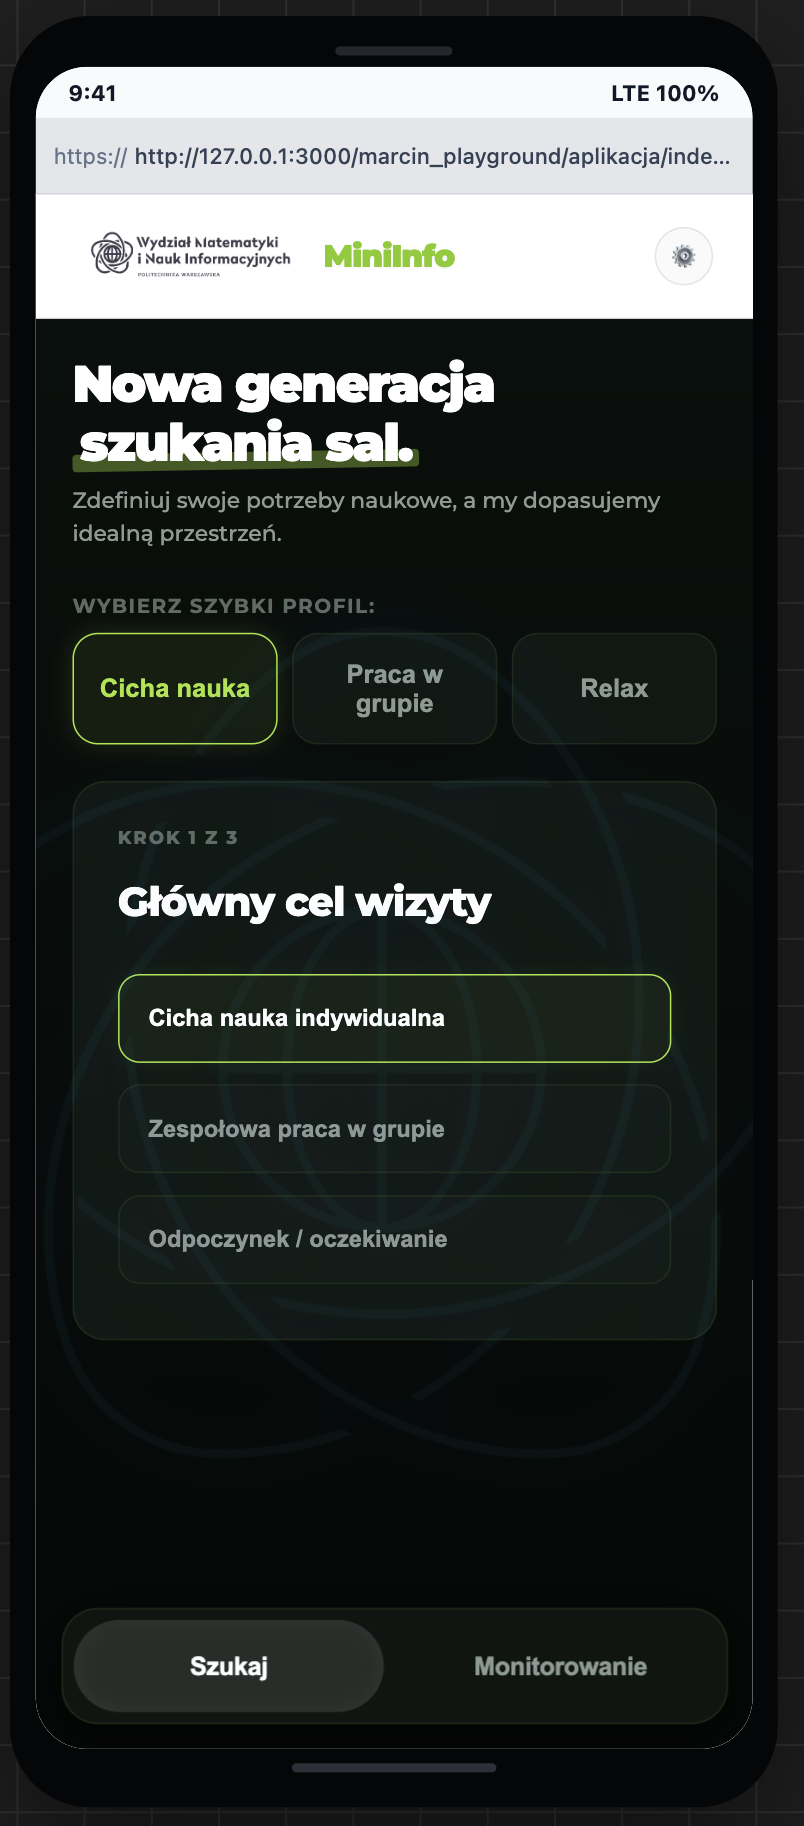
\includegraphics[width=\linewidth]{../raport4/r2/quiz.png}
        \caption{Ekran ankiety profilującej w~aplikacji MiniInfo.}
        \label{fig:app_ankieta5}
    \end{minipage}\hfill
    \begin{minipage}{0.47\textwidth}
        \centering
        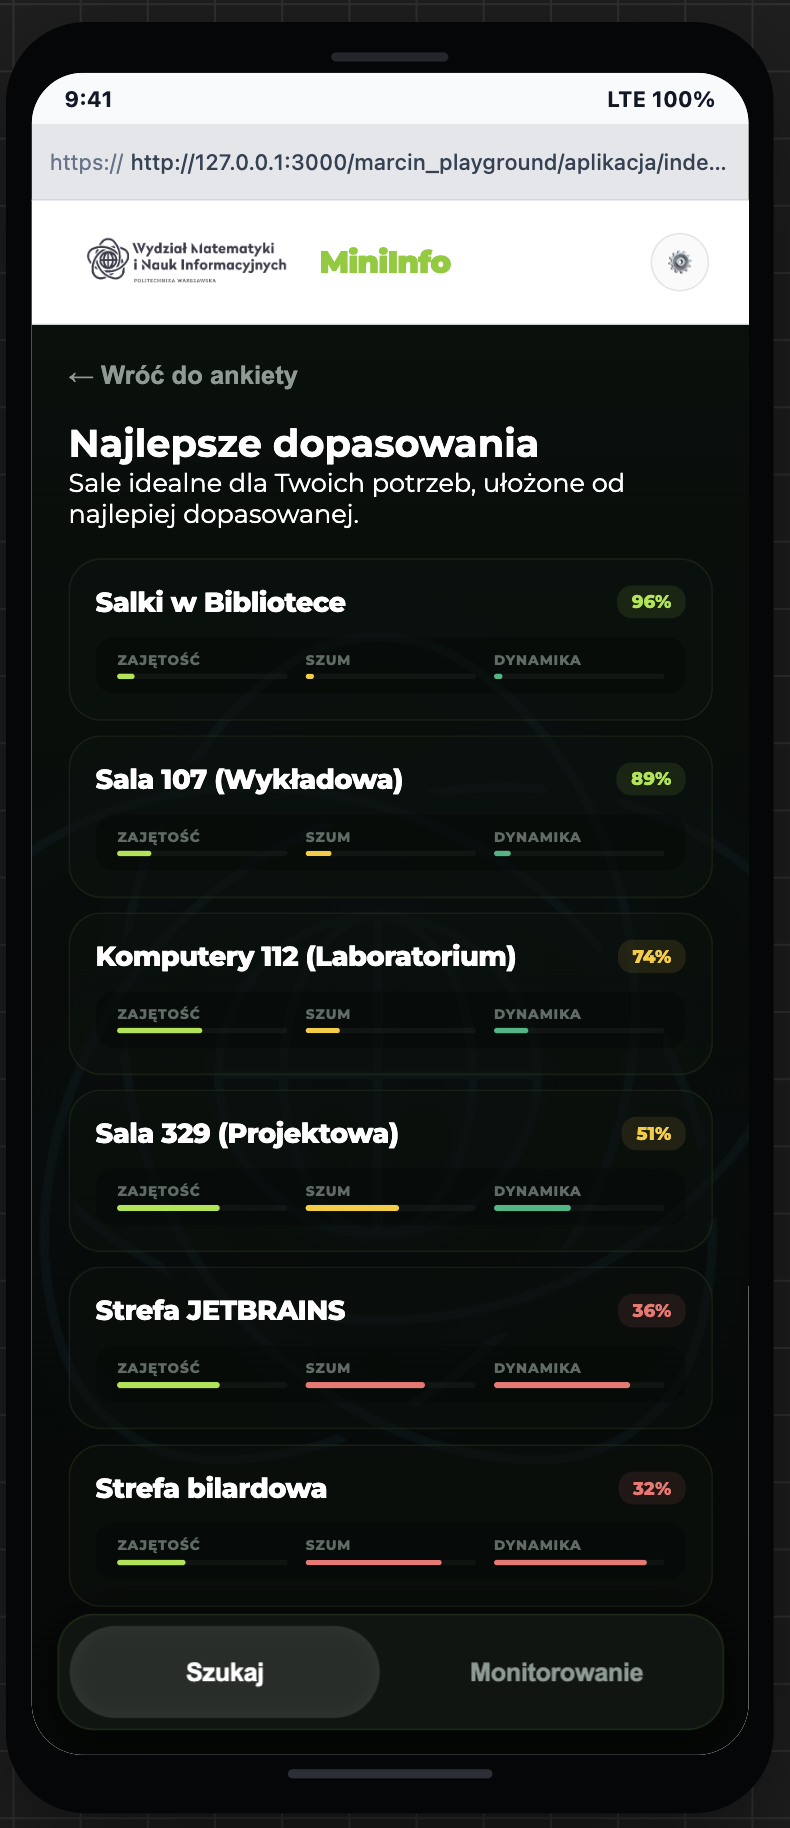
\includegraphics[width=\linewidth]{../raport4/r2/wynik.png}
        \caption{Ranking sal z~procentem dopasowania do profilu.}
        \label{fig:app_wyniki5}
    \end{minipage}
\end{figure}

\subsection{Przebieg procesu ankiety zwrotnej}

Diagram~\ref{fig:flowchart} przedstawia pełny przebieg procesu od momentu zgłoszenia problemu do aktualizacji wyników wyszukiwania.

\begin{figure}[H]
    \centering
    \tikzstyle{startstop} = [rectangle, rounded corners, minimum width=3.2cm, minimum height=0.9cm, text centered, draw=black, fill=teal!20, font=\small]
    \tikzstyle{process} = [rectangle, minimum width=3.5cm, minimum height=0.9cm, text centered, draw=black, fill=orange!15, font=\small]
    \tikzstyle{decision} = [diamond, minimum width=2.5cm, minimum height=1cm, text centered, draw=black, fill=yellow!20, font=\small, aspect=2.5]
    \tikzstyle{arrow} = [-{Stealth[length=3mm]}, thick]

    \begin{tikzpicture}[node distance=1.3cm]
        \node (start) [startstop] {Użytkownik odwiedza salę};
        \node (q1) [decision, below=of start] {Zadowolony?};
        \node (tak) [startstop, right=2.5cm of q1] {Sesja zamknięta (OK)};
        \node (nie) [process, below=of q1] {Wskazanie przyczyny};
        \node (check) [decision, below=of nie] {$\geq 3$ zgłoszenia?};
        \node (wait) [process, right=2.5cm of check] {Zgłoszenie zapisane};
        \node (median) [process, below=of check] {Oblicz medianę zgłoszeń};
        \node (update) [process, below=of median] {Aktualizuj dane sali};
        \node (rocchio) [process, below=of update] {Korekta Rocchio ($\vec{q}$, $\vec{w}$)};
        \node (rerun) [startstop, below=of rocchio] {Przelicz ranking};

        \draw [arrow] (start) -- (q1);
        \draw [arrow] (q1) -- node[above] {\footnotesize Tak} (tak);
        \draw [arrow] (q1) -- node[right] {\footnotesize Nie} (nie);
        \draw [arrow] (nie) -- (check);
        \draw [arrow] (check) -- node[above] {\footnotesize Nie} (wait);
        \draw [arrow] (check) -- node[right] {\footnotesize Tak} (median);
        \draw [arrow] (median) -- (update);
        \draw [arrow] (update) -- (rocchio);
        \draw [arrow] (rocchio) -- (rerun);
    \end{tikzpicture}
    \caption{Przebieg procesu ankiety zwrotnej --- od zgłoszenia do aktualizacji rankingu.}
    \label{fig:flowchart}
\end{figure}

\subsection{Mechanizm przetwarzania feedbacku}

Negatywny feedback przetwarza się dwuetapowo:

\textbf{1. Brama mediany (zabezpieczenie przed nadużyciami).} Pojedyncze zgłoszenie nie zmienia danych sali. Dopiero gdy co najmniej 3~niezależne osoby zgłoszą problem dla tej samej sali, system oblicza medianę z~ich zgłoszeń i~uruchamia korektę. Mediana (zamiast średniej) chroni przed fałszywymi skargami i~jednorazowymi anomaliami.

\textbf{2. Korekta wektora zapytania (algorytm Rocchio).} Jeśli użytkownik zgłosi, że w~sali było za głośno, system automatycznie:
\begin{itemize}
    \item zwiększa wagę parametru szumu: $w_S \leftarrow \min(1.0,\; w_S + 0.15)$,
    \item przesuwa wartość docelową szumu w~dół:
    \begin{equation}
        q_S \leftarrow \max(0.0,\; q_S - 0.35 \cdot S_i)
    \end{equation}
    gdzie $S_i$ to aktualny poziom szumu w~zgłoszonej sali, a~$\beta = 0.35$ to kara za błąd.
\end{itemize}

Po korekcie system natychmiast przelicza ranking i~proponuje alternatywną, cichszą salę. Dzięki temu aplikacja \emph{uczy się} na błędach i~z~czasem lepiej dopasowuje się do konkretnego użytkownika.

\subsection{Przykładowy scenariusz}

Student szuka ciszy przed egzaminem. Aplikacja poleca salę~432 z~dopasowaniem $89\%$. Po wejściu okazuje się, że w~sali odbywa się spotkanie grupowe. Student zgłasza: ,,Nie'' $\rightarrow$ ,,Za głośno''. Reakcja systemu:
\begin{enumerate}
    \item Zgłoszenie zapisane do kolejki dla sali 432.
    \item Jeśli to trzecie zgłoszenie w~krótkim czasie --- system aktualizuje poziom szumu sali na podstawie mediany.
    \item Waga ciszy dla tego użytkownika wzrasta ($w_S: 1.0 \rightarrow 1.0$, $q_S: 0.0 \rightarrow 0.0$, ale priorytet ciszy się potwierdza).
    \item Kolejne wyszukiwanie pominie salę 432 i~zaproponuje cichszą alternatywę (np.~pokój~537).
\end{enumerate}

% ============================================================
\section{Podsumowanie projektu MiniInfo}
% ============================================================

To ostatni raport z~projektu. Podsumowujemy uczciwie: co naprawdę zrobiliśmy, co działało, co nie, i~czego się nauczyliśmy.

\subsection{Co nam się udało}

\begin{itemize}
    \item \textbf{Działająca aplikacja webowa.} Zbudowaliśmy od zera aplikację mobilną (HTML/CSS/JS) działającą w~przeglądarce na telefonie. Użytkownik może wypełnić ankietę, zobaczyć ranking sal i~przejść do wybranej sali --- bez instalacji czegokolwiek.

    \item \textbf{Algorytm rankingowy.} Ważona odległość Euklidesowa w~przestrzeni $[0,1]^3$ daje sensowne wyniki. System mierzy dopasowanie sali do profilu matematycznie, a~nie przez proste filtrowanie.

    \item \textbf{Trzy profile użytkownika.} Ankieta 3-krokowa zamienia subiektywne preferencje na konkretne wektory zapytań $\vec{q}$ i~wagi $\vec{w}$. Profile ,,Cicha nauka'', ,,Praca w~grupie'' i~,,Relax'' pokrywają najczęstsze scenariusze na wydziale.

    \item \textbf{Sprzężenie zwrotne (Rocchio).} Mechanizm korekty po negatywnym feedbacku jest zaimplementowany i~działa --- system adaptuje się do użytkownika.

    \item \textbf{Dynamiczna aktualizacja danych.} System w~tle cyklicznie pobiera nowe odczyty z~czujników i~odświeża indeks sal. Drobne zmiany (wejście/wyjście pojedynczych osób) rejestrowane są co minutę, większe przesunięcia --- w~dłuższych interwałach.

    \item \textbf{Zabezpieczenie --- brama mediany.} Feedback od pojedynczego użytkownika nie zmienia danych sali. Dopiero 3~niezależne zgłoszenia uruchamiają korektę, a~system bierze medianę --- nie średnią.

    \item \textbf{Dwa eksperymenty z~prawdziwymi użytkownikami.} Testowaliśmy aplikację łącznie na ponad 50~osobach (45~w~Etapie~4, 12~w~Etapie~5). Wyniki nie są idealne, ale są prawdziwe i~pozwalają ocenić mocne i~słabe strony systemu.

    \item \textbf{Kompletna dokumentacja.} Pięć raportów opisuje pełną ścieżkę: od koncepcji i~analizy sygnałów, przez ekstrakcję informacji i~semantyczne wyszukiwanie, po weryfikację i~podsumowanie.
\end{itemize}

\subsection{Co nie działało lub okazało się niepotrzebne}

\begin{itemize}
    \item \textbf{Brak integracji z~planem zajęć USOS.} Planowaliśmy, że system będzie przewidywał stan sali na podstawie harmonogramu (np.~że za 20~minut skończy się wykład i~sala zostanie opanowana przez grupę). Nie wdrożyliśmy tego --- to największa funkcjonalna luka projektu.

    \item \textbf{Zbyt dużo teorii w~raportach.} W~Raportach~2 i~3 poświęciliśmy wiele stron opisowi sensorów mmWave, entropii, kompresji i~filtracji --- zamiast skupić się na tym, co aplikacja naprawdę robi. Prowadzący słusznie to zauważył.

    \item \textbf{Podobieństwo kosinusowe.} Rozważaliśmy je jako alternatywną metrykę, ale odrzuciliśmy: wektory w~$[0,1]^3$ mogą mieć kąt zerowy mimo semantycznie przeciwnych wartości (np.~$[0.1,0.1,0.1]^T$ vs.~$[0.9,0.9,0.9]^T$). Ważona odległość Euklidesowa okazała się lepsza.

    \item \textbf{Opóźnienie aktualizacji danych.} Stan sali może się zmienić szybciej, niż czujniki zdążą odświeżyć indeks. W~eksperymencie 2~z~4~negatywnych ocen wynikały właśnie z~tego opóźnienia.

    \item \textbf{Panel diagnostyczny (suwaki).} Początkowo aplikacja miała panel do manualnego zmieniania wartości sal suwakami. Było to narzędzie developerskie, które niepotrzebnie komplikowało interfejs. Zastąpiliśmy go mechanizmem zgłaszania błędów.

    \item \textbf{Ograniczona liczba czujników.} System monitoruje tylko 7~sal, a~czujniki nie uwzględniają wszystkich czynników środowiskowych (np.~bliskość głośnego korytarza, przenikanie dźwięku przez ściany). To ograniczenie wymaga dalszej kalibracji.
\end{itemize}

\subsection{Co było ciekawe i~czego się nauczyliśmy}

\begin{itemize}
    \item \textbf{Subiektywność jest mierzalna.} Na początku projektu nie było oczywiste, że da się zamienić preferencje typu ,,chcę ciszy'' na liczby i~dobrze posortować wyniki. Okazało się, że prosta ankieta + ważona metryka wystarczą do sensownych rekomendacji.

    \item \textbf{Profil ,,Relax'' jest łatwy, ,,Cicha nauka'' --- trudny.} Wynikło to empirycznie z~obu eksperymentów. Algorytm dobrze radzi sobie z~luźnymi preferencjami; gorzej z~rygorystycznymi wymaganiami absolutnej ciszy.

    \item \textbf{Mediana jest lepszą barierą niż próg.} Decyzja o~użyciu mediany zamiast prostego licznika zgłoszeń chroni przed fałszywymi alarmami i~celowym manipulowaniem danymi.

    \item \textbf{Prosta aplikacja mobilna może działać bez backendu.} Wszystko, co zbudowaliśmy, działa po stronie klienta --- bez serwera, bez bazy danych w~chmurze. To znacząco upraszcza deployment na wydziale.

    \item \textbf{Jakość danych > jakość algorytmu.} Nasz algorytm rankingowy działa poprawnie, ale jego skuteczność jest ograniczona przez jakość danych wejściowych. Nawet najlepszy wzór nie pomoże, jeśli dane nie odzwierciedlają rzeczywistości.
\end{itemize}

\subsection{Bilans projektu w~punktach}

\begin{table}[H]
    \centering
    \caption{Bilans projektu MiniInfo: plusy i~minusy.}
    \label{tab:bilans}
    \resizebox{\textwidth}{!}{
    \begin{tabular}{|p{7.5cm}|p{7.5cm}|}
        \hline
        \textbf{Plusy (+)} & \textbf{Minusy ($-$)} \\
        \hline
        Działająca aplikacja webowa (HTML/CSS/JS) & Ograniczona liczba monitorowanych sal \\
        \hline
        Algorytm ważonej odległości Euklidesowej & Brak integracji z~USOS \\
        \hline
        3~profile użytkownika z~ankietą & Za dużo teorii w~raportach 2--3 \\
        \hline
        Mechanizm Rocchio (feedback adaptacyjny) & Opóźnienie aktualizacji danych \\
        \hline
        Brama mediany (ochrona przed nadużyciami) & Mała próba w~eksperymencie (12~osób) \\
        \hline
        Dynamiczna aktualizacja z~czujników & Brak analizy widma dźwięku (mowa vs. szum) \\
        \hline
        2~eksperymenty z~prawdziwymi użytkownikami & Aplikacja działa tylko lokalnie \\
        \hline
        Pełna dokumentacja (5~raportów) & Tylko 7~sal w~indeksie \\
        \hline
    \end{tabular}
    }
\end{table}

\subsection{Kierunki dalszego rozwoju}

Gdyby projekt był kontynuowany, priorytetem byłyby:

\begin{enumerate}
    \item \textbf{Integracja z~planem zajęć USOS} --- system mógłby przewidywać stan sali na najbliższe godziny na podstawie harmonogramu.
    \item \textbf{Większa sieć czujników} --- więcej radarów mmWave i~mikrofonów zainstalowanych w~kolejnych salach na wydziale.
    \item \textbf{Personalizacja historyczna} --- system pamięta historię wyborów użytkownika i~z~czasem lepiej dopasowuje rekomendacje bez konieczności powtarzania ankiety.
    \item \textbf{Rozszerzenie indeksu sal} --- aktualnie 7~sal; na wydziale jest ich znacznie więcej.
    \item \textbf{Analiza widma dźwięku} --- rozróżnienie mowy (uciążliwa) od szumu tła (akceptowalny), co znacząco poprawiłoby trafność dla profilu ,,Cicha nauka''.
\end{enumerate}

% ============================================================
\section*{Podział prac}
% ============================================================
\begin{itemize}
    \item Eksperyment weryfikacyjny i~analiza wyników -- Iga Oleksiewicz, Maks Młynarczyk
    \item Mechanizm ankiety w~aplikacji i~feedback -- Marcin Pawlak, Ignacy Drężek
    \item Podsumowanie projektu i~wnioski -- Goran Pangełow, Mikołaj Pesta, Marcin Pawlak
    \item Redakcja techniczna i~kompilacja \LaTeX{} -- Mikołaj Pesta, Goran Pangełow
\end{itemize}

\end{document}
